\section{Design of the LNA}

In this section, we present the design methodology of the LNA architecture shown in Figure~\ref{fig:schem-lna}. The design focuses on transistor biasing and dimensioning to meet the specified gain, noise figure, and impedance matching requirements.

The topology combines a common-gate (CG) stage in parallel with a common-source (CS) stage at the input. The total input impedance is given by:
\[
Z_\text{in} = Z_\text{CG} \parallel Z_\text{CS}
\]
Since the CS stage ideally presents infinite input impedance, the overall impedance is primarily defined by the CG stage. Therefore, it is designed to match the standard \SI{50}{\ohm} source.

\label{sec:inpCap}
At high frequencies, however, parasitic capacitances become non-negligible. Even though smaller technologies have lower intrinsic capacitances, this is counterbalanced by the fact that they operate at higher frequencies—thus the capacitive reactance becomes comparable or dominant, influencing the input impedance and bandwidth.

The design workflow began with theoretical calculations using the square-law MOSFET model to estimate $g_m$, $I_D$, and $W/L$. These values were computed using a Python script and then verified in LTSpice simulations. The `.op` analysis allowed extraction of parameters like $g_{ds}$ and $g_{mb}$, which were otherwise difficult to estimate accurately. Based on this data, transistor sizes were refined iteratively to meet specifications.

\label{sec:assumptions}
During the initial calculations, the following assumptions were made:
\begin{itemize}
    \item $g_{ds} \ll g_m$, allowing simplification of gain expressions.
    \item $g_{mb} \approx 0.2\,g_m$, a typical approximation in short-channel MOSFETs.
    \item Overdrive voltage was fixed at $V_{DSsat} = \SI{100}{\milli\volt}$.
\end{itemize}

The following expressions were used to derive $g_m$ and $I_D$:
\begin{equation}
    g_m = \sqrt{2K_{n,p}\frac{W}{L}I_D} = \frac{2I_D}{V_{DSsat}} 
    \label{eq:gm_eq}
\end{equation}

\begin{equation}
    I_D = \frac{K_n}{2} \cdot \frac{W}{L} V_{DSsat}^2 
    \label{eq:ID_eq}
\end{equation}

Additionally, $g_{ds}$ was considered to follow the empirical trend:
\[
g_{ds} \propto \frac{1}{L}
\]
as supported by~\cite{AnalogCircDesign}.

\subsection{Common Gate Stage Design}

The CG small-signal equivalent circuit is shown in Figure~\ref{fig:CG_SmallSignal}. The relevant expressions for gain and input impedance are:

\begin{equation}
    A_v = \frac{v_o}{v_i} = \frac{g_m + g_{mb} + g_{ds}}{g_{ds} + \frac{1}{r_1}}
    \label{eq:CG_Gain}
\end{equation}

\begin{equation}
    Z_{in} = \frac{1}{g_m + g_{mb}} \quad \text{(approximation assuming $g_{ds} \ll g_m$)}
    \label{eq:CG_Zin}
\end{equation}

\begin{figure}[H]
    \centering
    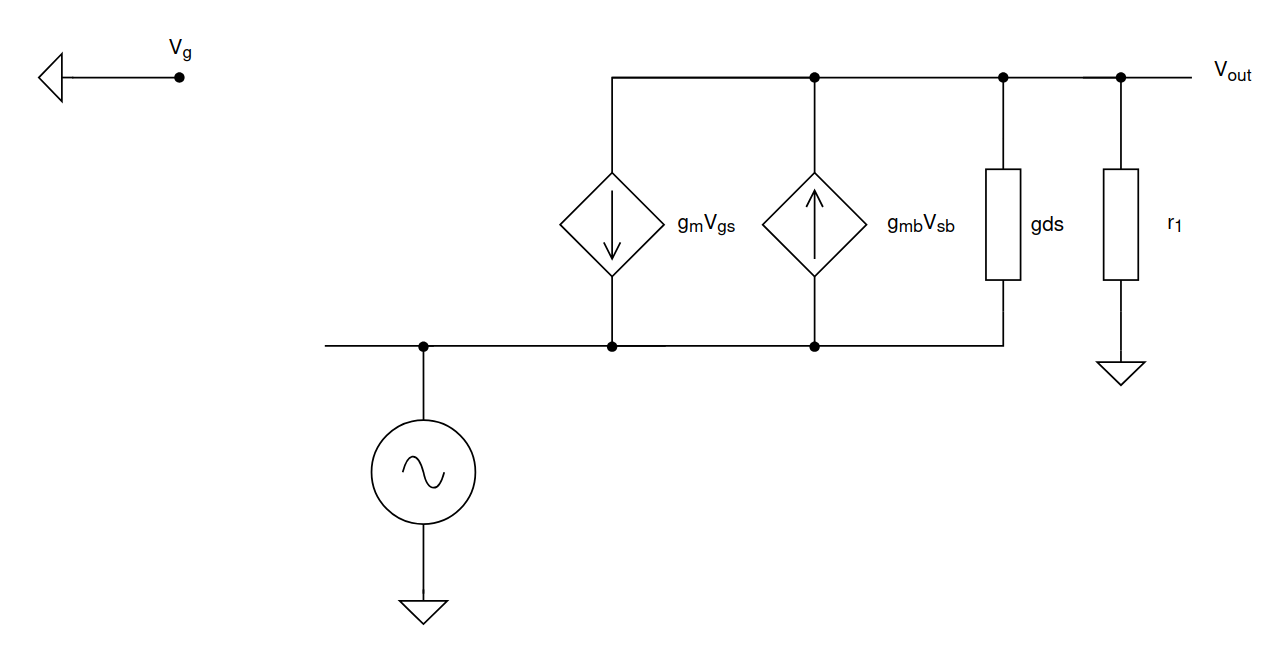
\includegraphics[width=0.8\textwidth]{Images/CG_SmallSignal.png}
    \caption{Small-signal equivalent circuit of the common-gate stage.}
    \label{fig:CG_SmallSignal}
\end{figure}
\subsubsection{Circuit Sizing}

To match $Z_{in} = \SI{50}{\ohm}$, and assuming $g_{mb} = 0.2\,g_m$, we compute:
\[
g_m = \frac{1}{Z_{in}(1 + 0.2)} \approx \SI{16.667}{\milli\siemens}
\]

Using $g_m$ and $V_{DSsat} = \SI{100}{\milli\volt}$:
\[
I_D = \frac{g_m \cdot V_{DSsat}}{2}
\]

Then $W/L$ is calculated using Equation~\ref{eq:ID_eq}. The resistor $r_1$ is adjusted to satisfy gain specifications via Equation~\ref{eq:CG_Gain}. Biasing voltages must ensure $V_S > 0$ and $V_S < V_D$, maintaining the MOSFET in saturation.

\subsection{Common Source Stage Design}

The CS small-signal schematic is shown in Figure~\ref{fig:CS_SmallSignal}. The voltage gain is given by:
\begin{equation}
    A_v = -g_m (r_{ds} \parallel R_L)
    \label{eq:CS_Gain}
\end{equation}

\begin{figure}[H]
    \centering
    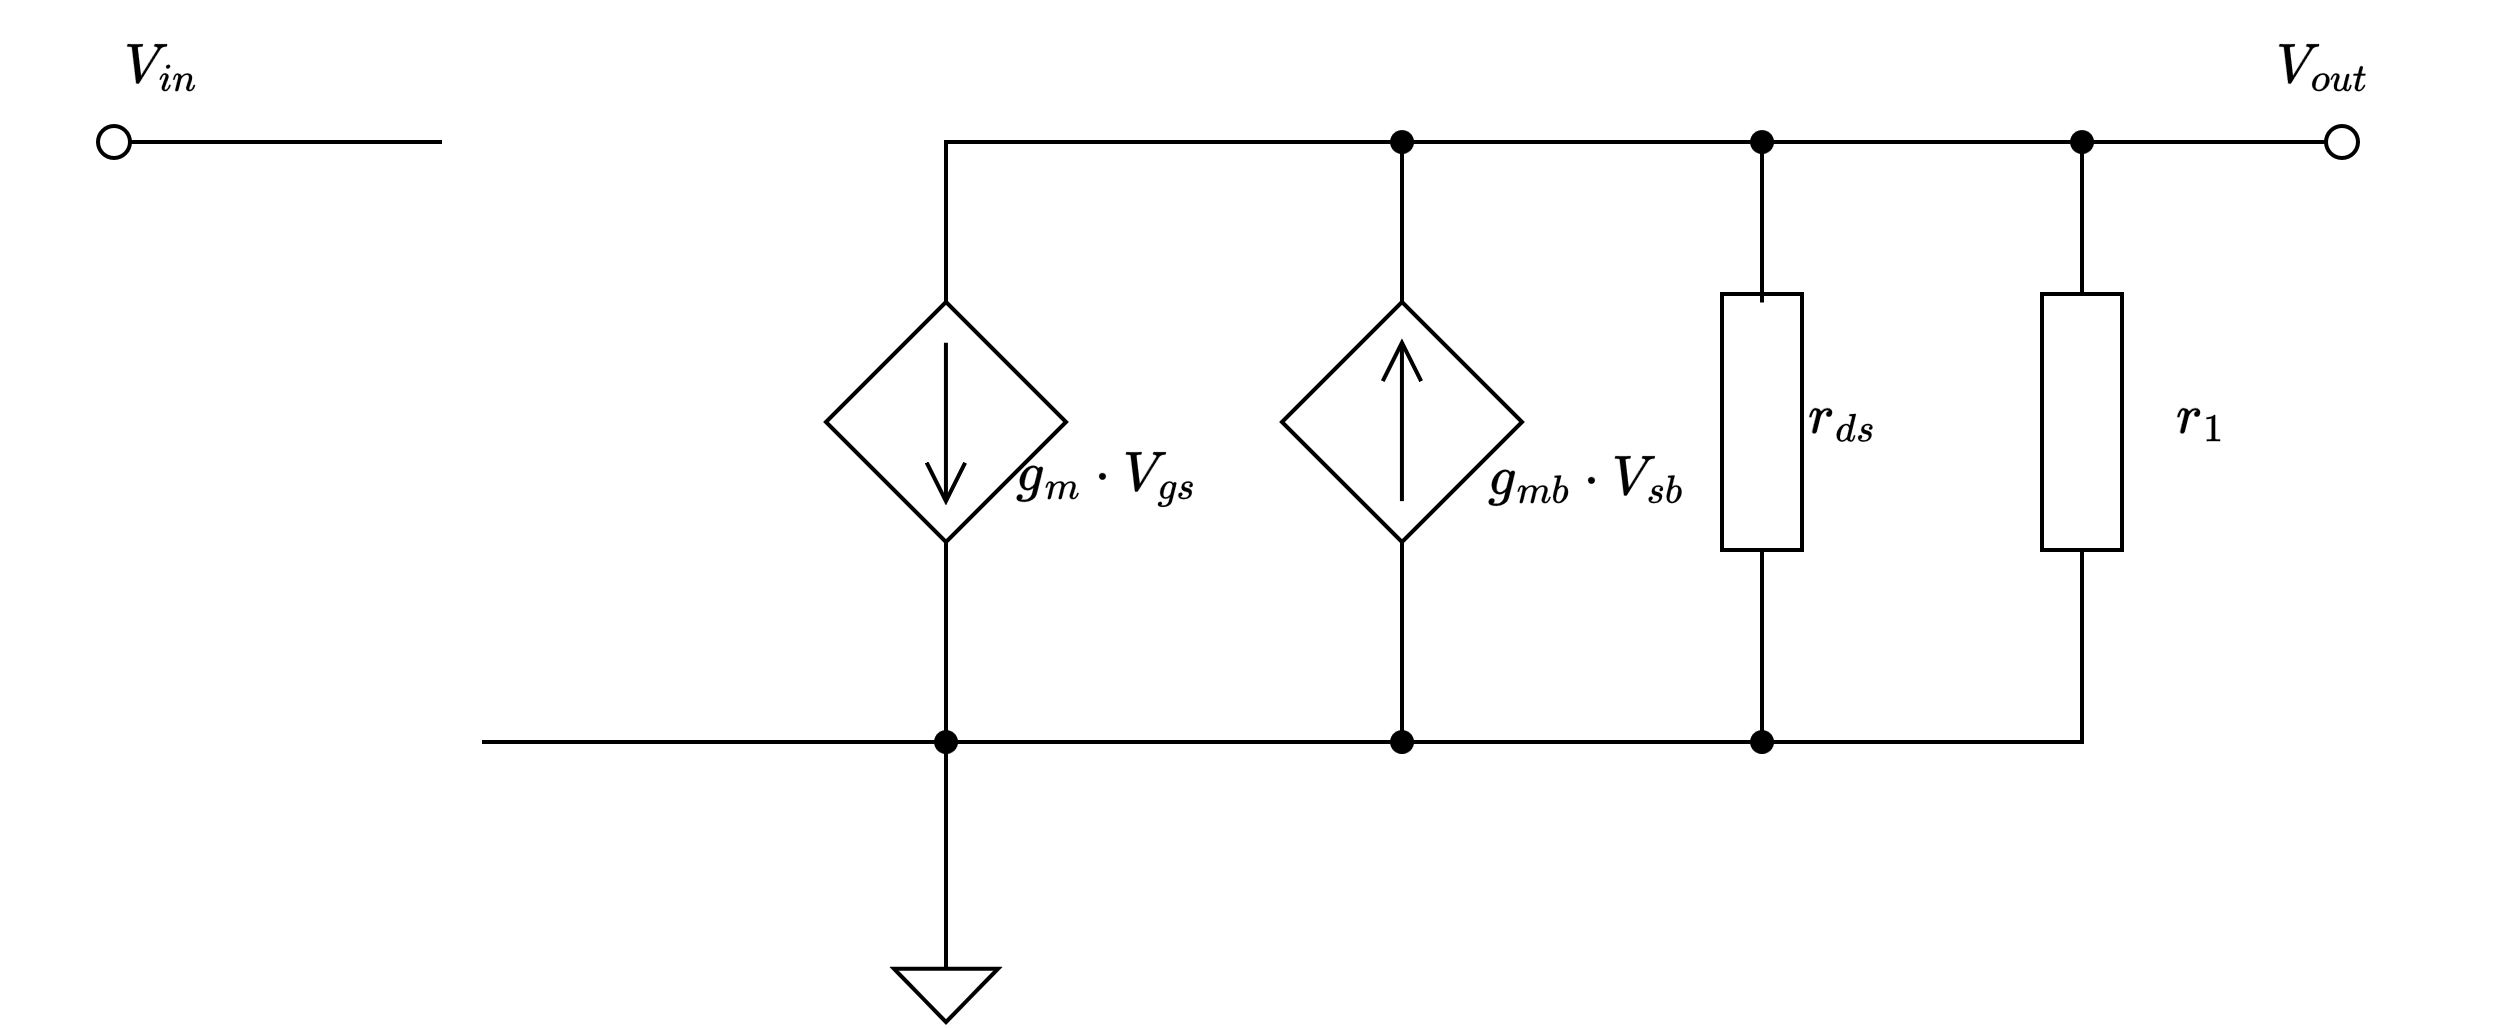
\includegraphics[width=0.8\textwidth]{Images/CS_SmallSig.png}
    \caption{Small-signal equivalent circuit of the common-source stage.}
    \label{fig:CS_SmallSignal}
\end{figure}

\subsubsection{Circuit Sizing}

Input impedance is not critical in the CS stage, but input capacitance still impacts high-frequency behavior (see Section~\ref{sec:inpCap}).

The $g_m$ is initially set equal to the CG stage, and later multiplied by $n = 3$ as required. Using Equation~\ref{eq:gm_eq}, we derive:
\begin{equation}
    \frac{W}{L} = \frac{g_{m}}{K_n V_{DSsat}} 
    \label{eq:wl2}
\end{equation}

To determine the load resistor $r_2$, we use:
\begin{equation}
    r_2 = -\frac{A_v \cdot r_{ds}}{A_v - g_m \cdot r_{ds}} 
    \label{eq:r2}
\end{equation}

Bias voltage is obtained as:
\begin{equation}
    V_{bias} = V_{GS} = V_{DSsat} + V_{th}
    \label{eq:V_bias_CS}
\end{equation}

\subsection{Buffer Stage Design}

The buffer stage schematic is shown in Figure~\ref{fig:Buff_SmallSignal}. Its gain and output impedance are approximated by:

\begin{equation}
    A_v \approx 1 + \frac{g_{m2}}{g_{m1}}
    \label{eq:buff_Gain}
\end{equation}

\begin{equation}
    Z_{out} \approx \frac{1}{g_{m1}} 
    \label{eq:buff_zout}
\end{equation}

Assuming $g_{m1} \gg g_{ds}$ and aiming for $Z_{out} \approx \SI{50}{\ohm}$, we require $g_{m1} \approx \SI{20}{\milli\siemens}$. Both $g_{m1}$ and $g_{m2}$ should be matched for symmetric gain.

Bias voltages are:
\[
V_{biasn} = V_{tn} + V_{DSsat}
\quad\text{and}\quad
V_{biasp} = \frac{V_{DD}}{2} + V_{GS}
\]

This ensures the output DC level is centered at $V_{DD}/2$.

\begin{figure}[H]
    \centering
    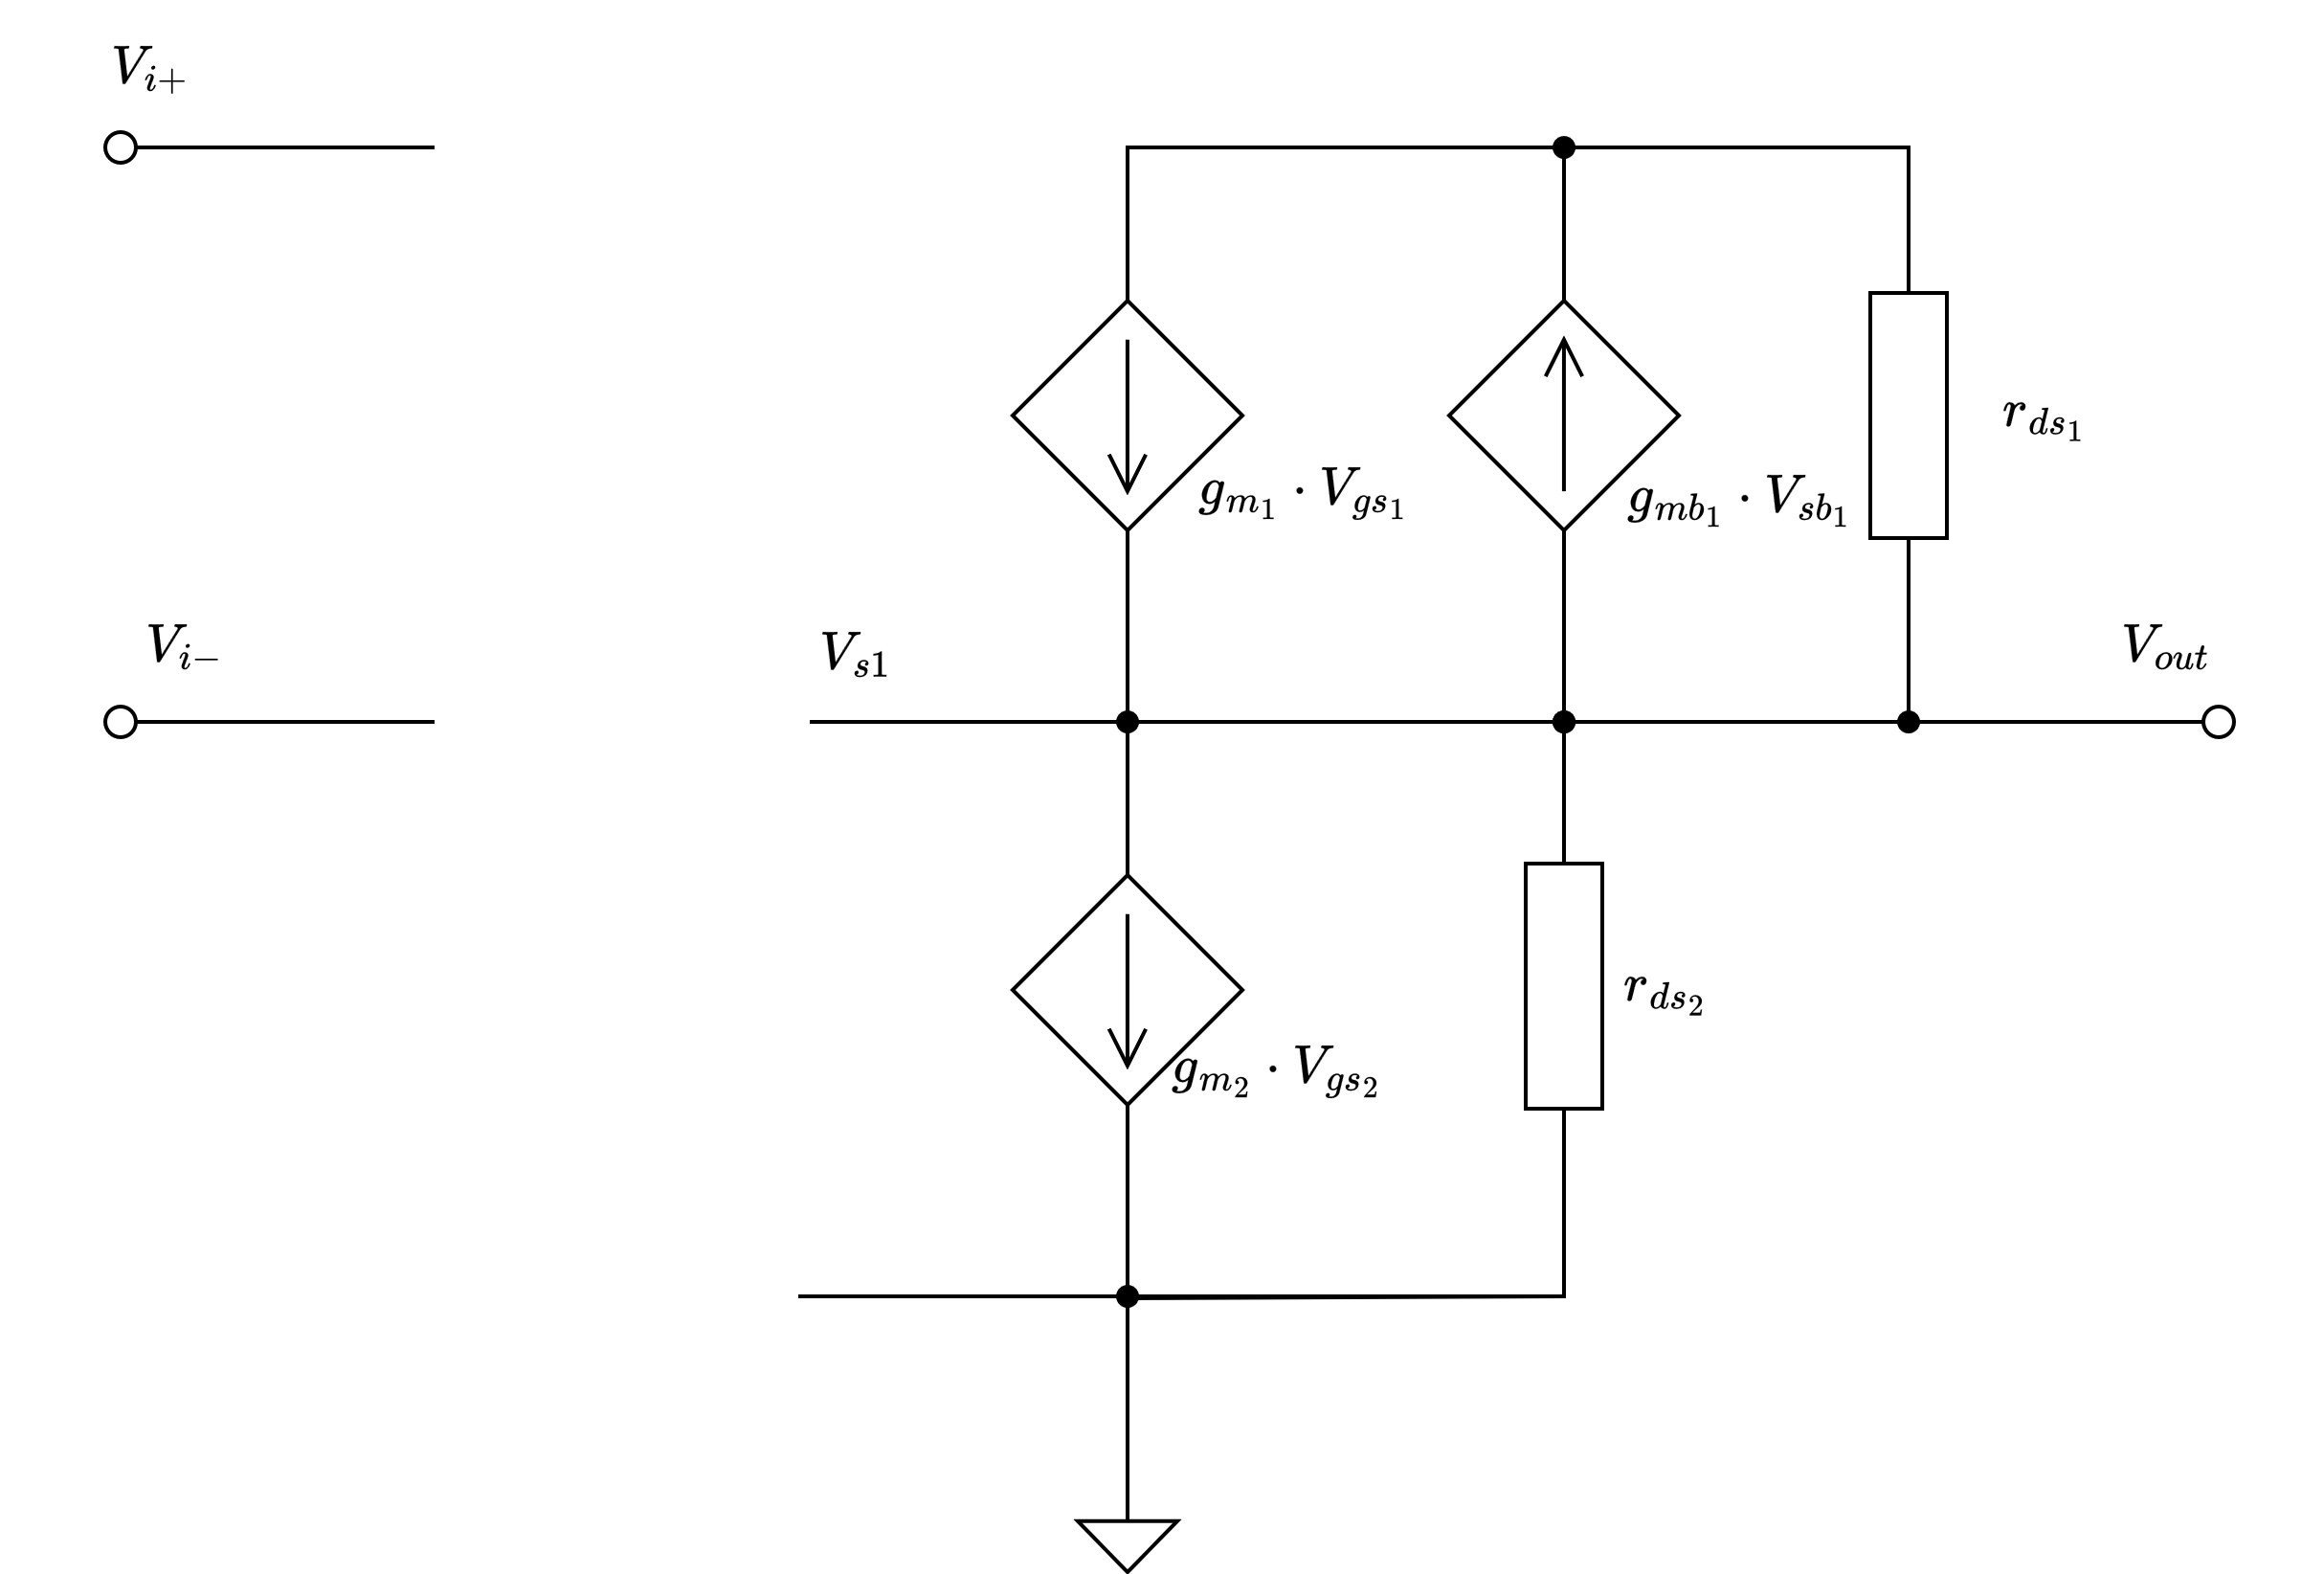
\includegraphics[width=0.7\textwidth]{Images/BufferSmallSignal.png}
    \caption{Small-signal equivalent circuit of the buffer stage.}
    \label{fig:Buff_SmallSignal}
\end{figure}

\subsection{Initial Values}

Initial values were calculated using the design equations and Python scripts. The results are summarized in Tables~\ref{tab:initial-vals-cg} and~\ref{tab:initial-vals-cs}.

\begin{table}[H]
    \centering
    \footnotesize
    \caption{Initial Values for the CG stage}
    \begin{tabularx}{\textwidth}{>{\centering\arraybackslash}X 
                                >{\centering\arraybackslash}X 
                                >{\centering\arraybackslash}X 
                                >{\centering\arraybackslash}X 
                                >{\centering\arraybackslash}X 
                                >{\centering\arraybackslash}X
                                >{\centering\arraybackslash}X}
        \toprule
        Node & $g_m$ ratio & W & L & $g_m$ (mS) & R ($\si{\ohm}$) & $V_{bias}$ (mV)  \\
        \midrule

        \multirow{1}{*}{350nm}
        &  1:1 & $\SI{291}{\micro\meter}$ & $\SI{350}{\nano\meter}$  & $15.9$ & $280$ & $1500$  \\

        \midrule
        \multirow{1}{*}{65nm}
        & 1:1 & \SI{108}{\micro\meter}  & \SI{65}{\nano\meter} & 16.7 & 278  & 350 \\
        
        \midrule
        \multirow{1}{*}{45nm}
        &  1:1 & \SI{642}{\micro\meter}  & \SI{135}{\nano\meter} & 17.3 & 286 & 352 \\


        \bottomrule
    \end{tabularx}
    \label{tab:initial-vals-cg}
\end{table}

\begin{table}[H]
    \centering
    \footnotesize
    \caption{Initial values for the CS stage}
    \begin{tabularx}{\textwidth}
        {@{}%  ⟵ trim left padding
         >{\centering\arraybackslash}X
         *{6}{>{\centering\arraybackslash}X}@{}} % ⟵ trim right padding
        \toprule
        Node & Config & W (\si{\micro\meter}) & L (\si{\nano\meter})
             & $g_m$ (mS) & R (\si{\ohm}) & $V_\text{bias}$ (mV) \\
        \midrule
        \multirow{2}{*}{\SI{350}{\nano\meter}}
            & 1:1 & \SI{291}{\micro\meter} & \SI{350}{\nano\meter} & 17.0 & 334 & 670 \\
            & 1:n & \SI{875}{\micro\meter} & \SI{350}{\nano\meter} & 51.8 &  103 & 700 \\
        \midrule
        \multirow{2}{*}{\SI{65}{\nano\meter}}
            & 1:1 & \SI{108}{\micro\meter} & \SI{65}{\nano\meter} & 16.7 & 334 & 400 \\
            & 1:n & \SI{325}{\micro\meter} & \SI{65}{\nano\meter} & 50.1 & 104 & 400 \\
        \midrule
        \multirow{2}{*}{\SI{45}{\nano\meter}}
            & 1:1 & \SI{450}{\micro\meter}  & \SI{135}{\nano\meter}  & 17.8 & 760 & 385 \\
            & 1:n & \SI{1350}{\micro\meter} & \SI{135}{\nano\meter} & 59.5 & 125 & 455 \\
        \bottomrule
    \end{tabularx}
    \label{tab:initial-vals-cs}
\end{table}

